\newpage
\section{Formel-Minimierung}
	
	\begin{multicols}{2}
	
		\subsection{Karnaugh-Maps}
			\begin{center}
				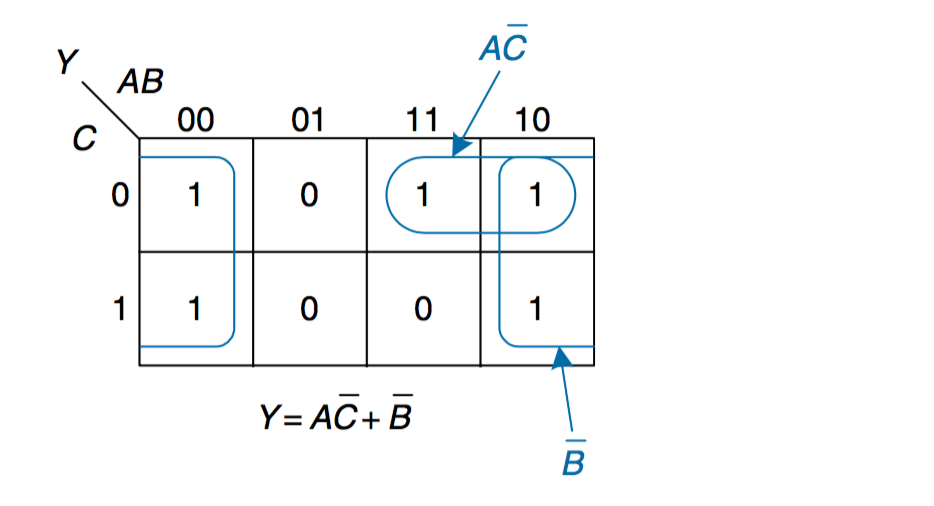
\includegraphics[width = 9cm]{images/minim/karnaugh}
			\end{center}
			You circle the biggest combination of one's possible with max length 2, and take the variables that don't change, karnaugh graphes work for functions with 4 or less variables.
		\subsection{Multiplexer}
			You can also write logic with a multiplexer. The selector of the multiplexer are your literals, the input of the multiplexer are one's for the input combination of your function, and zeros for the rest. To make the multiplexer smaller you can use a decoder.
			\paragraph{decoder}, in a decoder you make output of the multiplexer depend on a chosen literal, the High, to build a decoder it's easiest to use the truth tabel:
			\begin{center}
				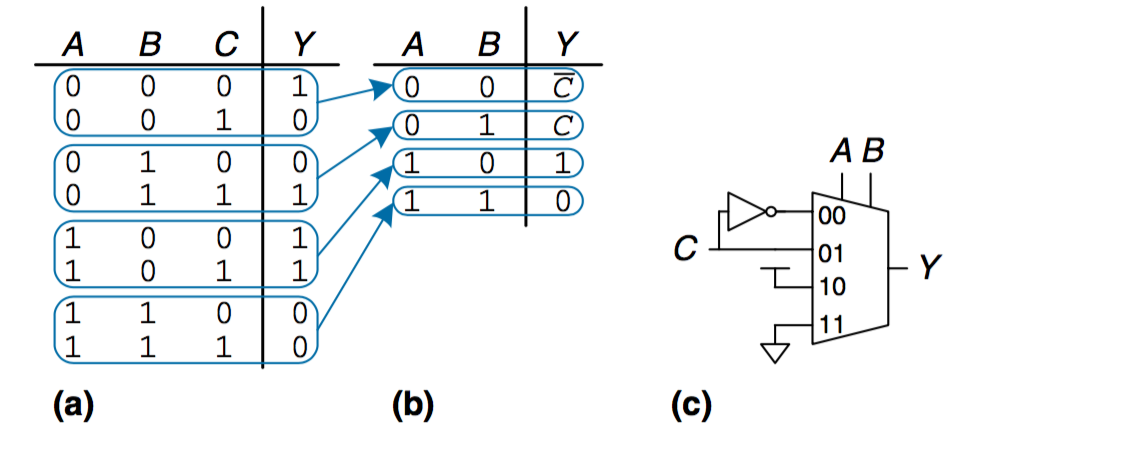
\includegraphics[width = 9cm]{images/minim/decoder}
			\end{center}			
	\end{multicols}






















